\documentclass{beamer}
\usepackage{amsmath}
\usepackage[english]{babel} %set language; note: after changing this, you need to delete all auxiliary files to recompile
\usepackage[utf8]{inputenc} %define file encoding; latin1 is the other often used option
\usepackage{csquotes} % provides context sensitive quotation facilities
\usepackage{graphicx} %allows for inserting figures
\usepackage{booktabs} % for table formatting without vertical lines
\usepackage{textcomp} % allow for example using the Euro sign with \texteuro
\usepackage{stackengine}
\usepackage{wasysym}
\usepackage{tikzsymbols}
\usepackage{textcomp}
\newcommand{\bubblethis}[2]{
        \tikz[remember picture,baseline]{\node[anchor=base,inner sep=0,outer sep=0]%
        (#1) {\underline{#1}};\node[overlay,cloud callout,callout relative pointer={(0.2cm,-0.7cm)},%
        aspect=2.5,fill=yellow!90] at ($(#1.north)+(-0.5cm,1.6cm)$) {#2};}%
    }%
\tikzset{face/.style={shape=circle,minimum size=4ex,shading=radial,outer sep=0pt,
        inner color=white!50!yellow,outer color= yellow!70!orange}}
%% Some commands to make the code easier
\newcommand{\emoticon}[1][]{%
  \node[face,#1] (emoticon) {};
  %% The eyes are fixed.
  \draw[fill=white] (-1ex,0ex) ..controls (-0.5ex,0.2ex)and(0.5ex,0.2ex)..
        (1ex,0.0ex) ..controls ( 1.5ex,1.5ex)and( 0.2ex,1.7ex)..
        (0ex,0.4ex) ..controls (-0.2ex,1.7ex)and(-1.5ex,1.5ex)..
        (-1ex,0ex)--cycle;}
\newcommand{\pupils}{
  %% standard pupils
  \fill[shift={(0.5ex,0.5ex)},rotate=80] 
       (0,0) ellipse (0.3ex and 0.15ex);
  \fill[shift={(-0.5ex,0.5ex)},rotate=100] 
       (0,0) ellipse (0.3ex and 0.15ex);}

\newcommand{\emoticonname}[1]{
  \node[below=1ex of emoticon,font=\footnotesize,
        minimum width=4cm]{#1};}
\usepackage{scalerel}
\usetikzlibrary{positioning}
\usepackage{xcolor,amssymb}
\newcommand\dangersignb[1][2ex]{%
  \scaleto{\stackengine{0.3pt}{\scalebox{1.1}[.9]{%
  \color{red}$\blacktriangle$}}{\tiny\bfseries !}{O}{c}{F}{F}{L}}{#1}%
}
\newcommand\dangersignw[1][2ex]{%
  \scaleto{\stackengine{0.3pt}{\scalebox{1.1}[.9]{%
  \color{red}$\blacktriangle$}}{\color{white}\tiny\bfseries !}{O}{c}{F}{F}{L}}{#1}%
}
\usepackage{fontawesome} % Social Icons
\usepackage{epstopdf} % allow embedding eps-figures
\usepackage{tikz} % allows drawing figures
\usepackage{amsmath,amssymb,amsthm} %advanced math facilities
\usepackage{lmodern} %uses font that support italic and bold at the same time
\usepackage{hyperref}
\usepackage{tikz}
\hypersetup{
    colorlinks=true,
    linkcolor=blue,
    filecolor=magenta,      
    urlcolor=blue,
}
\usepackage{tcolorbox}
%add citation management using BibLaTeX
\usepackage[citestyle=authoryear-comp, %define style for citations
    bibstyle=authoryear-comp, %define style for bibliography
    maxbibnames=10, %maximum number of authors displayed in bibliography
    minbibnames=1, %minimum number of authors displayed in bibliography
    maxcitenames=3, %maximum number of authors displayed in citations before using et al.
    minnames=1, %maximum number of authors displayed in citations before using et al.
    datezeros=false, % do not print dates with leading zeros
    date=long, %use long formats for dates
    isbn=false,% show no ISBNs in bibliography (applies only if not a mandatory field)
    url=false,% show no urls in bibliography (applies only if not a mandatory field)
    doi=false, % show no dois in bibliography (applies only if not a mandatory field)
    eprint=false, %show no eprint-field in bibliography (applies only if not a mandatory field)
    backend=biber %use biber as the backend; backend=bibtex is less powerful, but easier to install
    ]{biblatex}
\addbibresource{../mybibfile.bib} %define bib-file located one folder higher


\usefonttheme[onlymath]{serif} %set math font to serif ones

\definecolor{beamerblue}{rgb}{0.2,0.2,0.7} %define beamerblue color for later use

%%% defines highlight command to set text blue
\newcommand{\highlight}[1]{{\color{blue}{#1}}}


%%%%%%% commands defining backup slides so that frame numbering is correct

\newcommand{\backupbegin}{
   \newcounter{framenumberappendix}
   \setcounter{framenumberappendix}{\value{framenumber}}
}
\newcommand{\backupend}{
   \addtocounter{framenumberappendix}{-\value{framenumber}}
   \addtocounter{framenumber}{\value{framenumberappendix}}
}

%%%% end of defining backup slides

%Specify figure caption, see also http://tex.stackexchange.com/questions/155738/caption-package-not-working-with-beamer
\setbeamertemplate{caption}{\insertcaption} %redefines caption to remove label "Figure".
%\setbeamerfont{caption}{size=\scriptsize,shape=\itshape,series=\bfseries} %sets figure  caption bold and italic and makes it smaller


\usetheme{Boadilla}

%set options of hyperref package
\hypersetup{
    bookmarksnumbered=true, %put section numbers in bookmarks
    naturalnames=true, %use LATEX-computed names for links
    citebordercolor={1 1 1}, %color of border around cites, here: white, i.e. invisible
    linkbordercolor={1 1 1}, %color of border around links, here: white, i.e. invisible
    colorlinks=true, %color links
    anchorcolor=black, %set color of anchors
    linkcolor=beamerblue, %set link color to beamer blue
    citecolor=blue, %set cite color to beamer blue
    pdfpagemode=UseThumbs, %set default mode of PDF display
    breaklinks=true, %break long links
    pdfstartpage=1 %start at first page
    }


% --------------------
% Overall information
% --------------------
\title[Principios de Economía]{Principios de Economía}
\date{}
\author[Ertola y Sturzenegger]{Gabriela Ertola y Federico Sturzenegger }
\vspace{0.4cm}
\institute[]{Universidad de San Andrés \\
2022} 


\begin{document}

\begin{frame}
\frametitle{Principios de Economía
\centering
\\ \vspace{12mm} Teoría del consumidor}
\centering 

\includegraphics[scale=0.25]{Figures/logoUDESA.jpg} 
\end{frame}

\begin{frame}
\frametitle{La economía, los modelos y las funciones}
\begin{itemize}
    \item La economía estudia cómo asignar recursos escasos de forma eficiente, y \vspace{2mm}
    \item Las funciones (y sus expresiones matemáticas y gráficas) nos ayudan a representar ideas... \vspace{2mm}
    \item ¿Cómo podemos utilizar funciones para crear un modelo de ESCASEZ en economía? 
    \begin{itemize}
        \item ¿Qué significa que los recursos son escasos? ¡No hay de todo para todos! 
    \end{itemize}
    \item Por lo tanto, aparece otro concepto importante para entender: las personas enfrentan trade-offs
\end{itemize} 
\end{frame}

\begin{frame}
\frametitle{Trade-off}
\begin{itemize}
    \item Tomar una decisión implica tener más de una alternativa \vspace{2mm}
    \item Pero los recursos son escasos...  \vspace{2mm}
    \item Entonces, la escasez representa básicamente una restricción o límite \vspace{2mm}
\end{itemize} 
\end{frame}

\begin{frame}
\frametitle{ Decisiones}
\begin{itemize}
    \item Cada vez que tomamos una decisión y elegimos algo, es que al hacerlo siempre ganamos algo pero también perdemos algo \vspace{2mm}
    \item ¿Cómo tomamos una decisión? 
    \begin{itemize}
        \item Evaluamos todos los beneficios que se obtienen por tomar la decisión y compararlos con todos los costos que resultan de la decisión (Regla 1)
        \item Elegimos aquella alternativa tal que los beneficios incrementales sean superiores a los costos incrementales (Regla 2)
        \vspace{1mm}
    \end{itemize}
    \item A veces es fácil pensar en esto, pero otras veces no tanto...
\end{itemize} 
\end{frame}

\begin{frame}
\frametitle{Beneficios y costos}
\begin{itemize}
    \item Los beneficios son aquellas cosas que ganamos \vspace{2mm}
    \item Los costos son aquellas cosas que perdemos \vspace{2mm}
    \item ¿Cómo podemos cuantificar los beneficios y los costos? 
    \begin{itemize}
    \item Cuando disponemos de "precios de mercado" se facilita la cuestión
    \item Pero cuando no, es mas difícil cuantificar y buscamos otras formas. Por ejemplo: ranking de preferencias
    \end{itemize}
\end{itemize} 
\end{frame}

\begin{frame}
\frametitle{ Cuando se trata de costo relevantes... }
\begin{itemize}
    \item  \href{https://econ.video/2017/08/28/the-simpsons-opportunity-cost-of-lines/}{El costo de oportunidad}
    \begin{itemize}
        \item El costo de oportunidad de una alternativa es el valor de lo que se renuncia al optar por esa alternativa
    \end{itemize}
    \vspace{2mm}
    \item La falacia del costo hundido.  
    \begin{itemize}
        \item Ocurre cuando se están considerando costos y beneficios que no varían con las consecuencias de su decisión
        \item Let it go!
    \end{itemize}
    \vspace{2mm}
    \item \href{https://www.goodfood.com.au/eat-out/good-food-guides/the-surprising-costs-of-running-a-restaurant-20180327-h0y23c}{Los costos escondidos} 
    \vspace{2mm}
\end{itemize} 
\end{frame}

%\begin{frame}
%\frametitle{6. Probemos algunos ejercicios en grupo}
%\begin{itemize}
%    \item ¿Por qué las heladeras tienen luz pero los freezers no?
%    \item ¿Por qué los huevos marrones son mas caros que los blancos si está demostrado que ni el gusto ni la calidad de nutricional del huevo depende de su color?
%    \item ¿Por qué los habitantes de zonas rurales se casan antes que los habitantes de las ciudades?
%    \item ¿Por qué se puede manejar hablando por tel con manos libres pero no se puede usar el tel?
%\end{itemize} 
%\end{frame}

\begin{frame}
\frametitle{La decisión de consumo}
\centering

\includegraphics[scale=0.9]{Figures/Tema_02.1_pizzabirra.jpg}
\end{frame}

\begin{frame}
\frametitle{ El problema del estudiante}
\centering
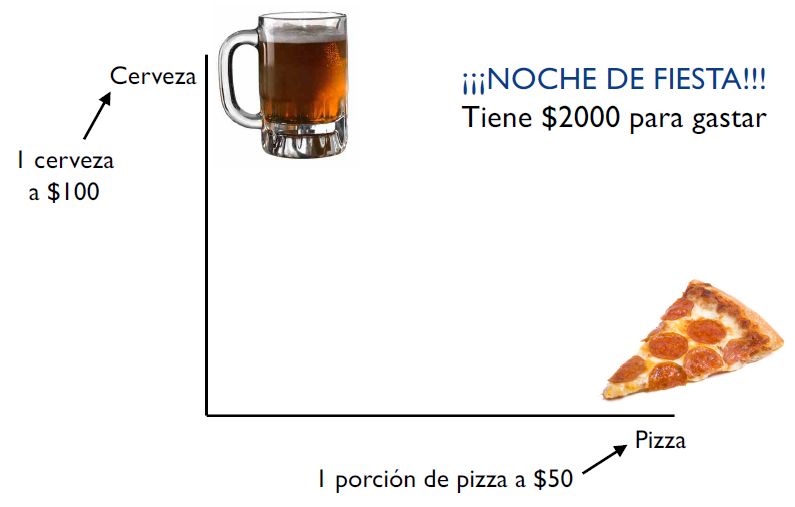
\includegraphics[scale=0.5]{Figures/Tema_02.2_rp.png}
\end{frame}

\begin{frame}
\frametitle{ El problema del estudiante}
\centering
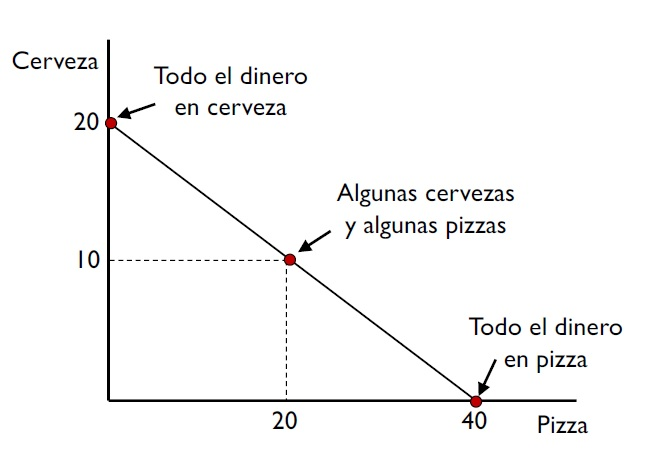
\includegraphics[scale=0.6]{Figures/Tema_02.3_rp1.jpg}
\end{frame}

\begin{frame}
\frametitle{Restricción presupuestaria}
\centering
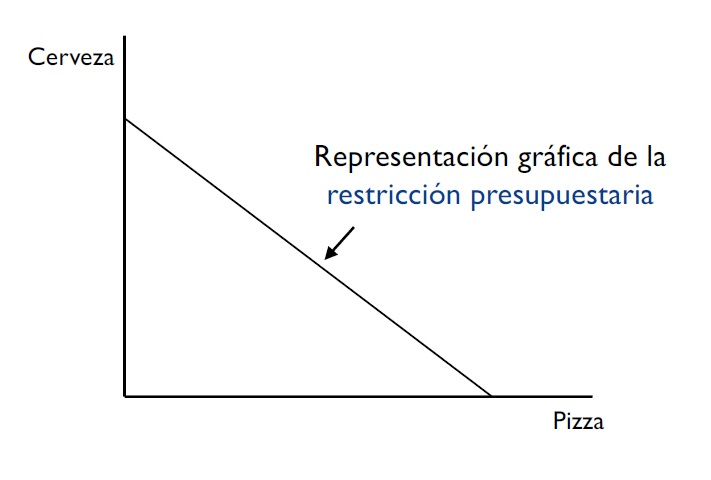
\includegraphics[scale=0.6]{Figures/Tema_02.4_rp2.jpg}
\end{frame}

\begin{frame}
\frametitle{1 ¿Cuánto puede consumir?}
\centering
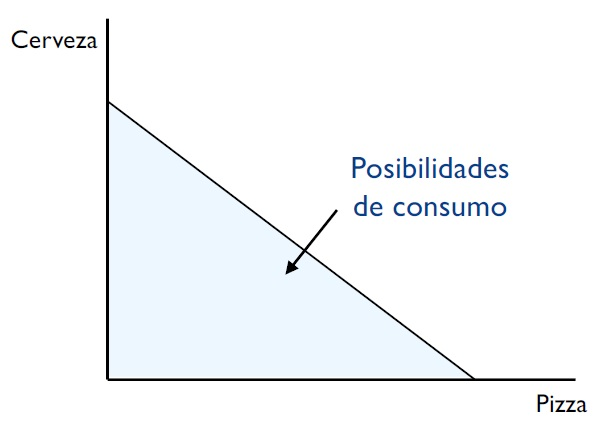
\includegraphics[scale=0.6]{Figures/Tema_02.5_rp3.jpg}
\end{frame}

\begin{frame}
\frametitle{El precio de la pizza}
\centering
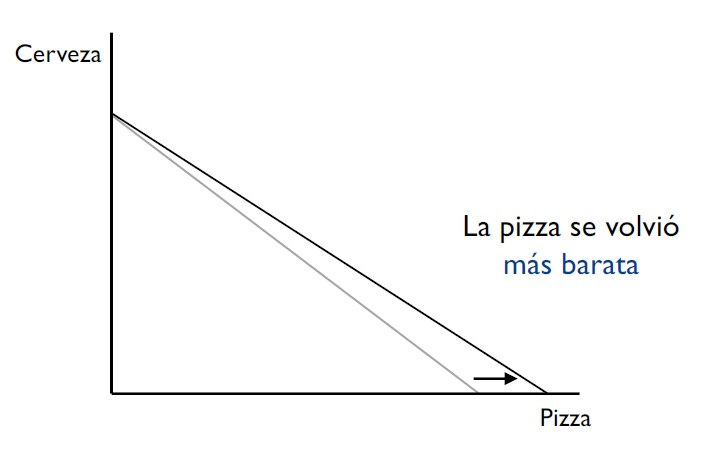
\includegraphics[scale=0.6]{Figures/Tema_02.6_rp4.jpg}
\end{frame}

\begin{frame}
\frametitle{El precio de la cerveza}
\centering
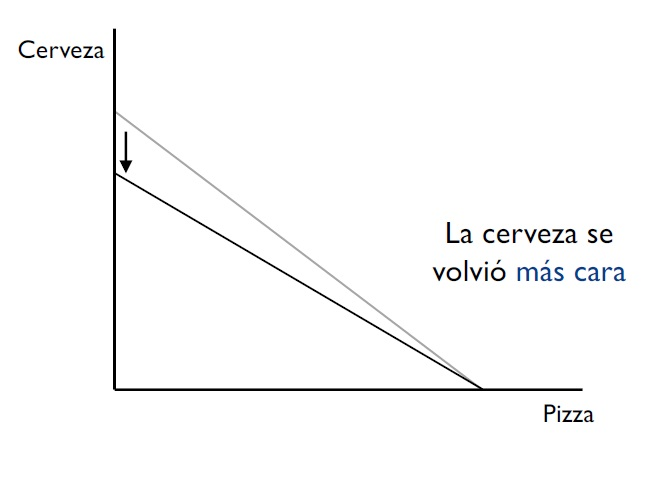
\includegraphics[scale=0.6]{Figures/Tema_02.7_rp5.jpg}
\end{frame}

\begin{frame}
\frametitle{Precios relativos}
\centering
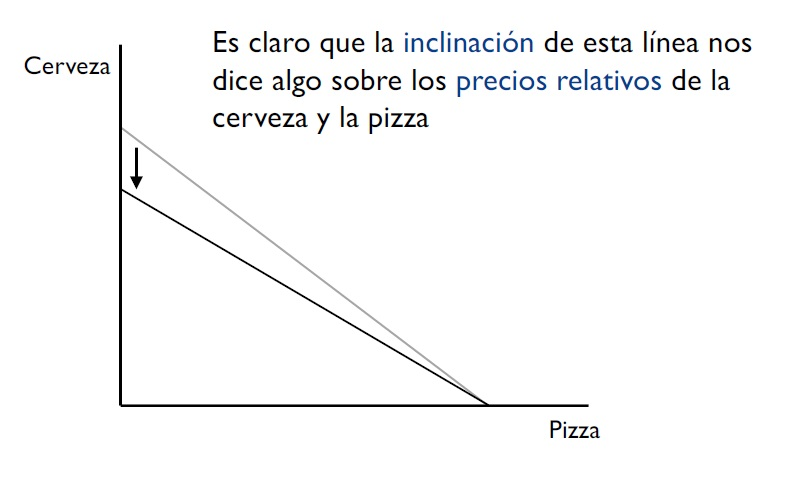
\includegraphics[scale=0.55]{Figures/Tema_02.8_rp6.jpg}
\end{frame}

\begin{frame}
\frametitle{Pendiente}
\begin{itemize}
    \item Llamamos "pendiente" a la inclinación de una función en un punto particular.
    \item En general, va a estar determinada por la distancia vertical con respecto a la distancia horizontal \\
    $Pendiente = \frac{\text{Distancia Vertical}}{\text{Distancia Horizontal}}$
    \item En el caso de la restricción presupuestaria del ejemplo, este ratio es constante a lo largo de la función, y va a estar dado por los precios relativos de la pizza
    $Pendiente = - \frac{\text{Precio Pizza}}{\text{Precio Cerveza}}= -\frac{P_{Pizza}}{P_{Cerveza}}=-\frac{P_P}{P_C}$
\end{itemize} 
\end{frame}

\begin{frame}
\frametitle{ Si rompemos el chanchito o vamos a la casa de la abuela...}
\centering
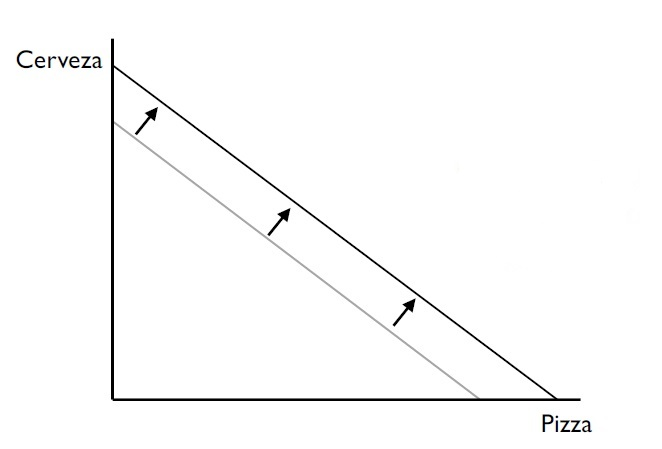
\includegraphics[scale=0.55]{Figures/Tema_02.9_rp7.jpg}
\end{frame}

\begin{frame}
\frametitle{ Recursos}
\centering
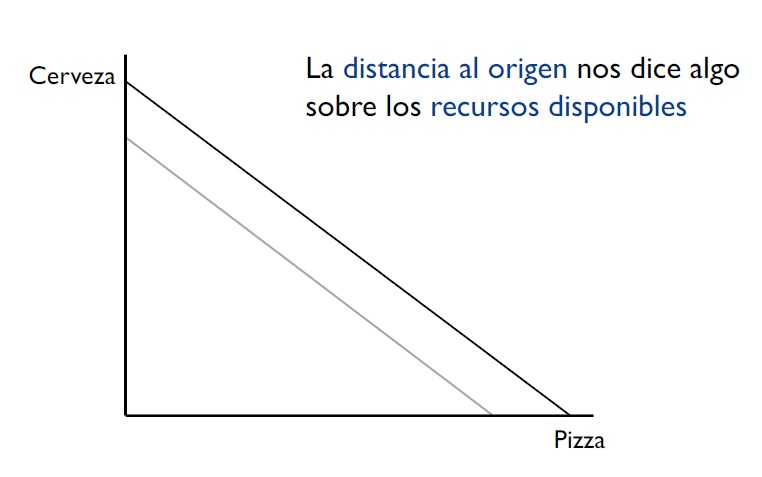
\includegraphics[scale=0.55]{Figures/Tema_02.10_rp8.jpg}
\end{frame}

\begin{frame}
\frametitle{ Restricción presupuestaria}
\begin{itemize}
    \item La representación gráfica de la restricción presupuestaria es útil para ver:
    \begin{itemize}
        \item Posibilidades de consumo
        \item Precios relativos de los bienes
    \end{itemize}
    \item Pero lo mismo se puede ver estudiando la expresión matemática \\
    $Ingresos$ = $P_{Cerveza} * Q_{Cerveza}$ + $P_{Pizza} * Q_{Pizza}$
    \\
    \item De hecho, las expresiones matemáticas pueden ser mas flexibles que las representaciones gráficas...
    \item Los economistas usan mucho ambas (junto con palabras), para construir modelos.
\end{itemize} 
\end{frame}


\begin{frame}
\frametitle{ Las preferencias}
\centering
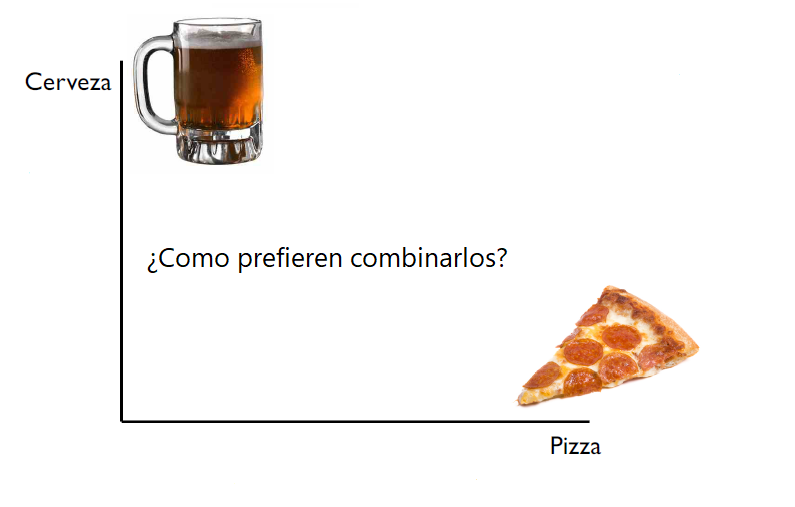
\includegraphics[scale=0.55]{Figures/Tema_02.11_rp9.png}
\end{frame}

\begin{frame}
\frametitle{ Distintas combinaciones...}
\centering
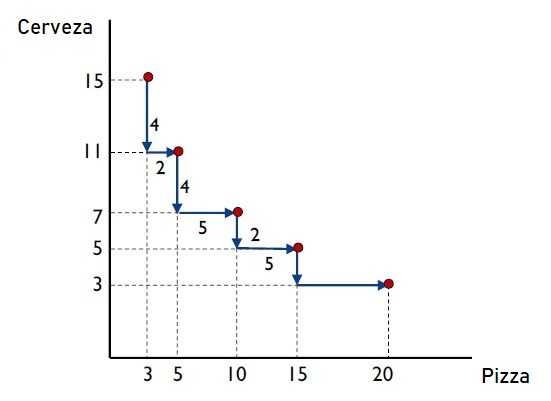
\includegraphics[scale=0.6]{Figures/Tema_02.12_rp10.jpg}
\end{frame}

\begin{frame}
\frametitle{ ...que me dejan igual de feliz}
\centering
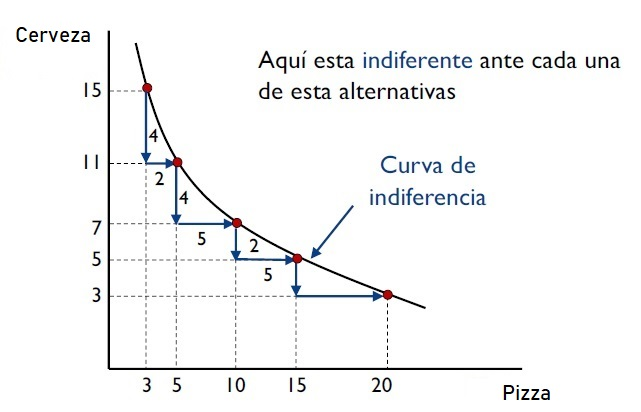
\includegraphics[scale=0.6]{Figures/Tema_02.13_rp11.jpg}
\end{frame}

\begin{frame}
\frametitle{Pero hay infinitas combinaciones...}
\centering
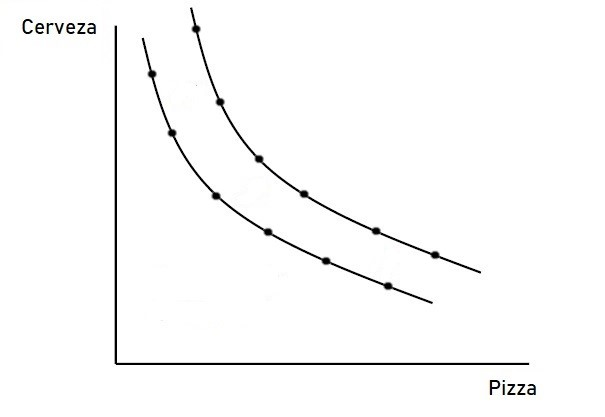
\includegraphics[scale=0.6]{Figures/Tema_02.15_rp12.jpg}
\end{frame}

\begin{frame}
\frametitle{ ... que podemos comparar}
\centering
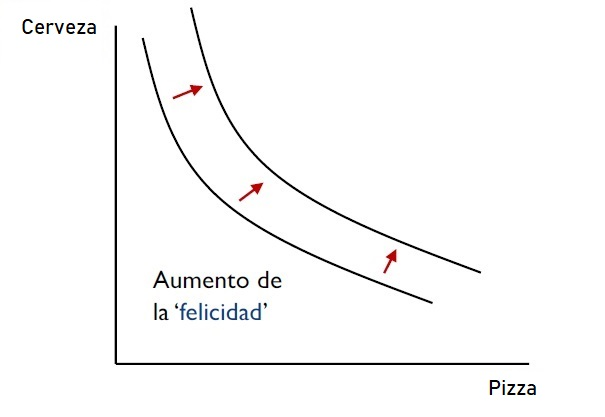
\includegraphics[scale=0.6]{Figures/Tema_02.15_rp13.jpg}
\end{frame}

\begin{frame}
\frametitle{ Y construimos un mapa de preferencias}
\centering
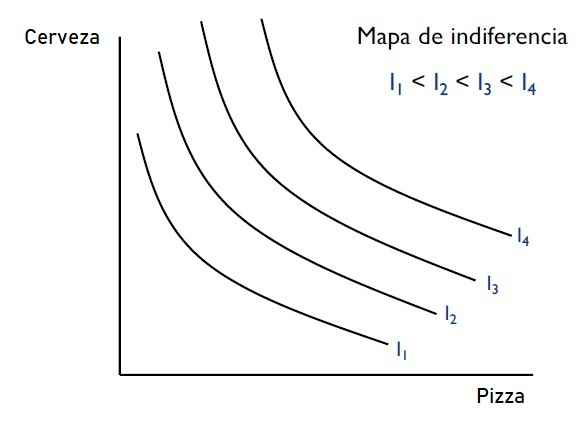
\includegraphics[scale=0.6]{Figures/Tema_02.16_rp14.jpg}
\end{frame}

\begin{frame}
\frametitle{ Las curvas de indiferencia}
\begin{itemize}
    \item Las curvas de indiferencia tienen pendiente negativa
    \item Las curvas de indiferencia más altas corresponden a niveles de utilidad más altos
    \item Las curvas de indiferencia son usualmente suaves: quiere decir que cambios pequeños en la cantidad de bienes no causan grandes saltos en utilidad
    \item Las curvas de indiferencia no se cruzan
    \item Las curvas de indiferencia se hacen más planas hacia la derecha y verticales a la izquierda
\end{itemize} 
\end{frame}

\begin{frame}
\frametitle{ Costo-beneficio}
\centering
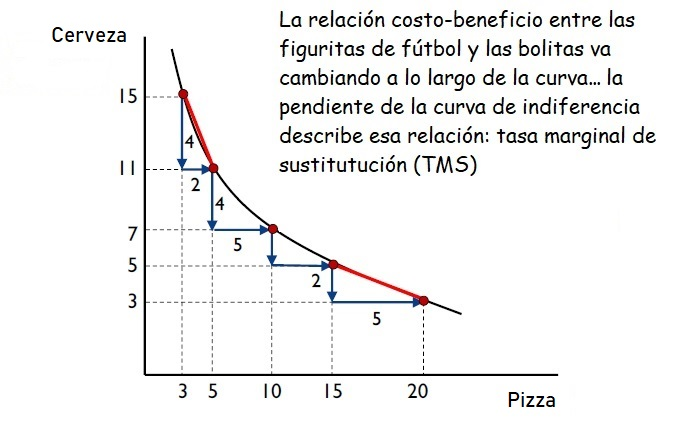
\includegraphics[scale=0.65]{Figures/Tema_02.17_rp15.jpg}
\end{frame}

\begin{frame}
\frametitle{ Comportamiento del consumidor}
\begin{itemize}
    \item Se puede entonces ver a los consumidores como individuos que tienen: \vspace{2mm}
    \begin{itemize}
        \item[1.] Recursos limitados \\
        - Por lo tanto, enfrentan una restricción presupuestaria \vspace{2mm}
        \item[2.] Ciertas preferencias sobre diferentes productos \\ \vspace{2mm}
    \end{itemize}
    \item También hacemos un supuesto adicional: \vspace{2mm}
    \begin{itemize}
    \item Los individuos son RACIONALES \\ \vspace{2mm}
    - ¿En qué forma se suele entender esto?
      \\ Que toman la mejor decisión posible dada la información
    \end{itemize}
\end{itemize} 
\end{frame}

\begin{frame}
\frametitle{ Volviendo al problema del estudiante}
\centering
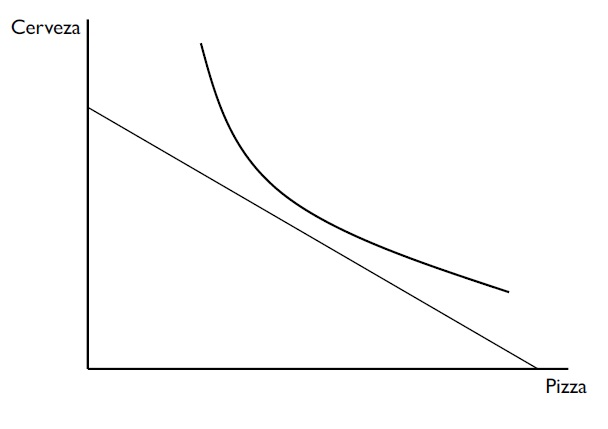
\includegraphics[scale=0.65]{Figures/Tema_02.18_rp16.jpg}
\end{frame}

\begin{frame}
\frametitle{ Equilibrio}
\centering
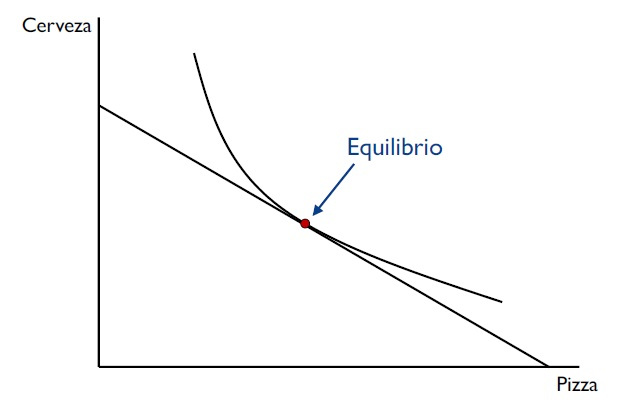
\includegraphics[scale=0.65]{Figures/Tema_02.19_rp17.jpg}
\end{frame}

\begin{frame}
\frametitle{Maximizando la utilidad}
\begin{itemize}
    \item Una idea central en economía es que las personas buscan maximizar su felicidad
    \\ \vspace{2mm}
    - En la jerga se dice que los individuos intentan ``maximizar su utilidad''. \\ \vspace{2mm}
    - La función de utilidad es la que describe cómo los bienes se traducen en utilidad: \vspace{2mm}
        \begin{itemize}
        Las curvas de indiferencia no son otra cosa que ``cortes'' de esa función para distintos niveles de utilidad
        \end{itemize}
    \item Habitualmente, expresamos y estudiamos este comportamiento con modelos matemáticos \\
    - ¿Tiene sentido?
\end{itemize} 
\end{frame}

\begin{frame}
\frametitle{ Tratemos de entender para que sirve pensar de este modo...}
\centering

\includegraphics[scale=0.5]{Figures/Tema_02.23_rp21.png}
\end{frame}

\begin{frame}
\frametitle{ Reacción a un shock de precios (ceteris paribus)}
\centering
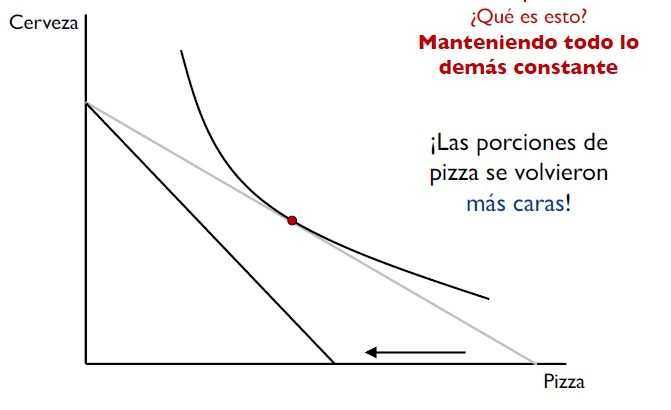
\includegraphics[scale=0.65]{Figures/Tema_02.20_rp18.jpg}
\end{frame}

\begin{frame}
\frametitle{ Reacción a un shock de precios (ceteris paribus)}
\centering
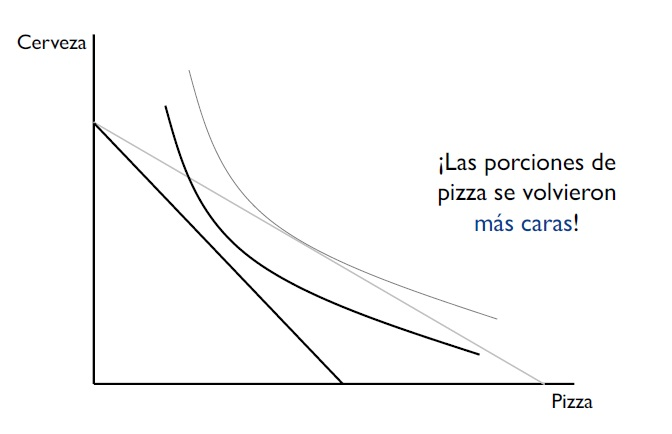
\includegraphics[scale=0.65]{Figures/Tema_02.21_rp19.jpg}
\end{frame}

\begin{frame}
\frametitle{Un nuevo equilibrio}
\centering
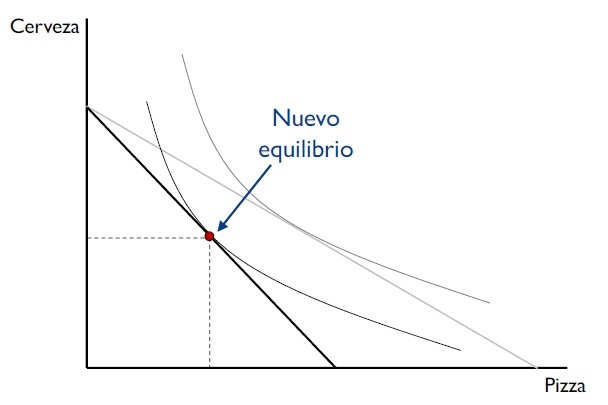
\includegraphics[scale=0.65]{Figures/Tema_02.22_rp20.jpg}
\end{frame}

\begin{frame}
\frametitle{ Curva Precio-Consumo}
\begin{itemize}
    \item Imaginemos que el precio de la pizza vuelve a aumentar ¿qué sucederá?  
    \item La curva Precio-Consumo muestra todas las mejores canastas asequibles 
\end{itemize}
\end{frame}

\begin{frame}
\frametitle{ Gráficamente}
\centering
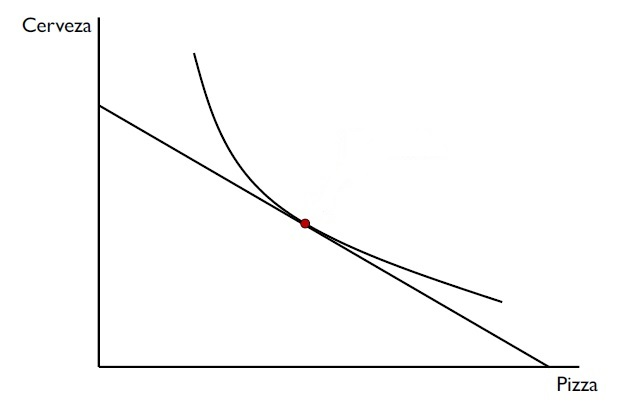
\includegraphics[scale=0.65]{Figures/Tema_02.22_rp21.jpg}
\end{frame}


\begin{frame}
\frametitle{Reacción a un shock de precios (ceteris paribus)}
\centering
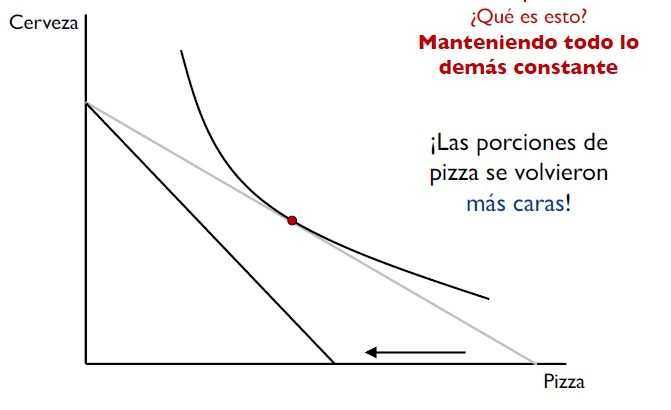
\includegraphics[scale=0.65]{Figures/Tema_02.20_rp18.jpg}
\end{frame}

\begin{frame}
\frametitle{Reacción a un shock de precios (ceteris paribus)}
\centering
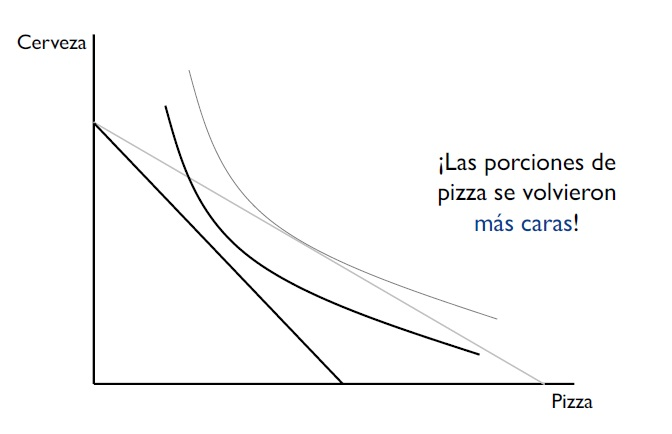
\includegraphics[scale=0.65]{Figures/Tema_02.21_rp19.jpg}
\end{frame}

\begin{frame}
\frametitle{Un nuevo equilibrio}
\centering
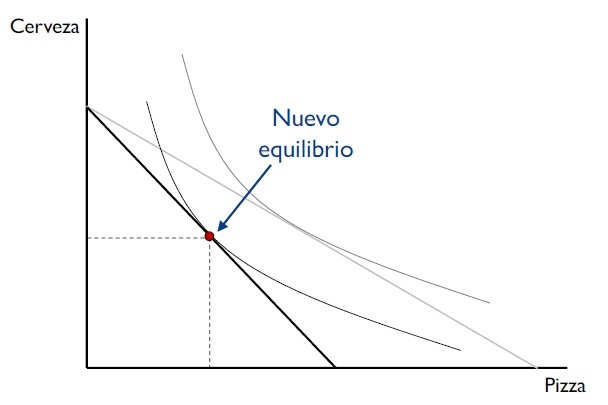
\includegraphics[scale=0.65]{Figures/Tema_02.22_rp20.jpg}
\end{frame}

\begin{frame}
\frametitle{Curva Precio-Consumo}
\begin{itemize}
    \item Imaginemos que el precio de la pizza vuelve a aumentar ¿qué sucederá?  
    \item La curva Precio-Consumo muestra todas las mejores canastas asequibles 
\end{itemize}
\end{frame}

\begin{frame}
\frametitle{Gráficamente}
\centering
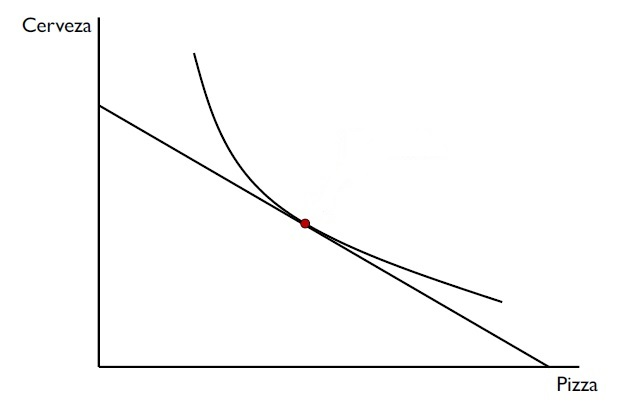
\includegraphics[scale=0.65]{Figures/Tema_02.22_rp21.jpg}
\end{frame}


\begin{frame}
\frametitle{¡Retomemos!}
\centering
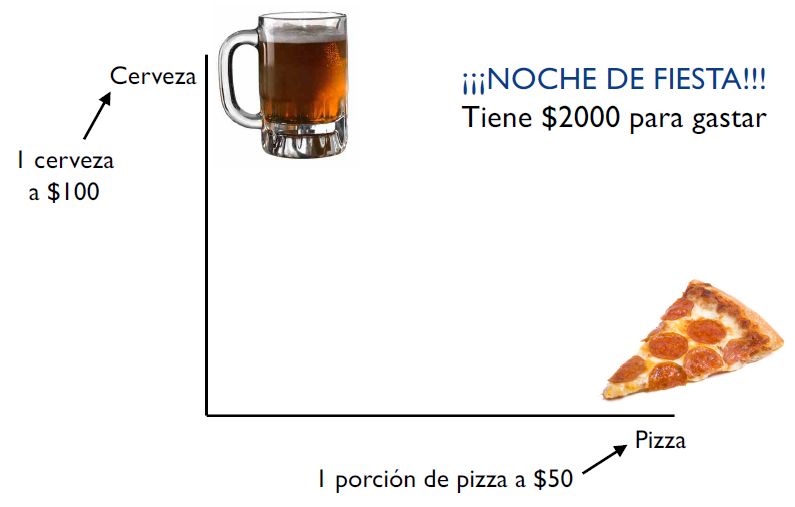
\includegraphics[scale=0.5]{Figures/Tema_02.2_rp.png}
\end{frame}

\begin{frame}
\frametitle{Tenemos la restricción presupuestaria}
\centering
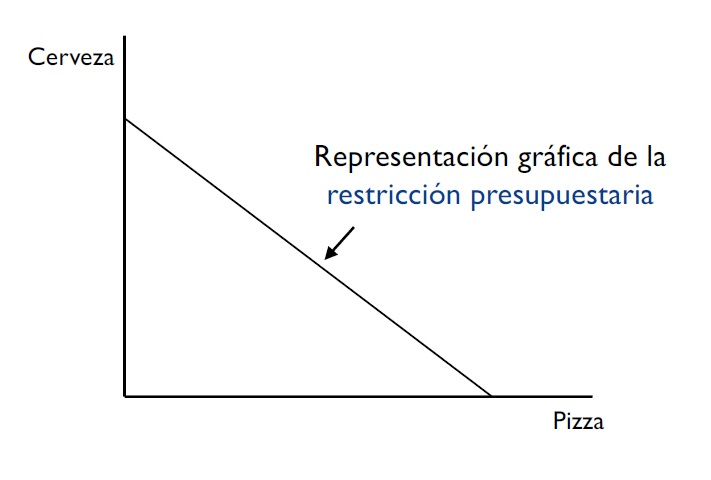
\includegraphics[scale=0.6]{Figures/Tema_02.4_rp2.jpg}
\end{frame}

\begin{frame}
\frametitle{ Agregamos las preferencias}
\centering
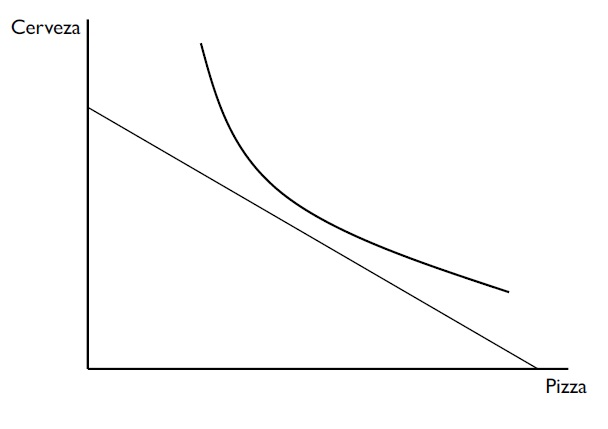
\includegraphics[scale=0.6]{Figures/Tema_02.18_rp16.jpg}
\end{frame}

\begin{frame}
\frametitle{ Y encontramos el equilibrio}
\centering
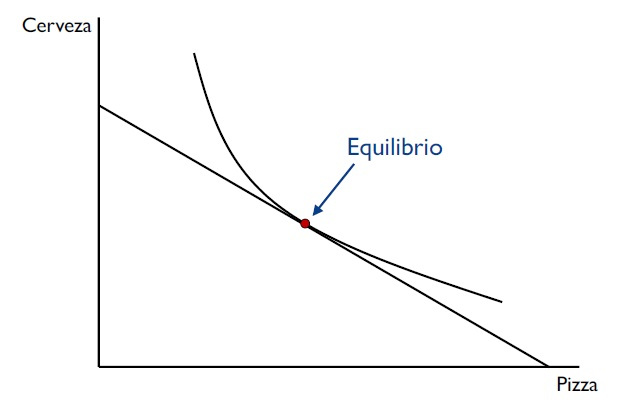
\includegraphics[scale=0.6]{Figures/Tema_02.19_rp17.jpg}
\end{frame}

\begin{frame}
\frametitle{ Cambios en los precios}
\begin{itemize}
    \item Si mantenemos constantes el ingreso del individuo y el precio de la cerveza, ¿cómo afectara un cambio en el precio de la pizza a la cantidad de pizza que adquiera el consumidor? \vspace{2mm}
    \begin{itemize}
         \item La canasta de bienes asequible es la que resulta de igualar la pendiente de la curva de indiferencia con la pendiente de la restricción presupuestaria 
    \end{itemize}
\end{itemize}
\end{frame}

\begin{frame}
\frametitle{ Tenemos un nuevo equilibrio}
\centering
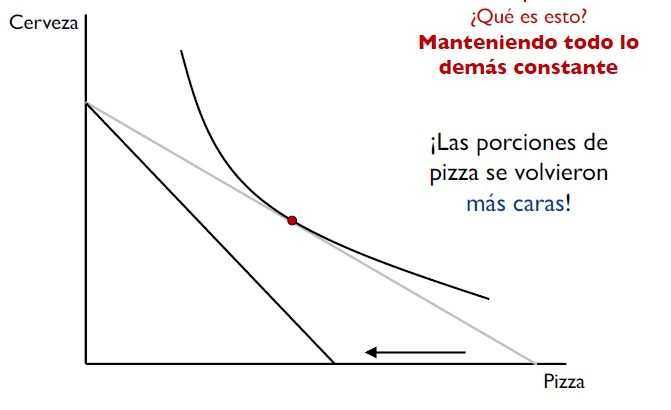
\includegraphics[scale=0.6]{Figures/Tema_02.20_rp18.jpg}
\end{frame}

\begin{frame}
\frametitle{ ¿Qué pasaba si cambiaban los precios?}
\centering
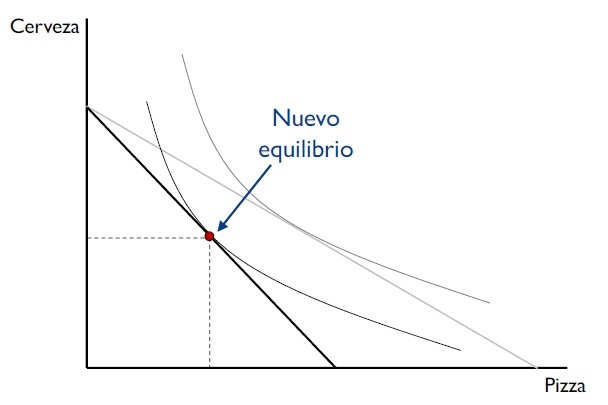
\includegraphics[scale=0.6]{Figures/Tema_02.22_rp20.jpg}
\end{frame}

\begin{frame}
\frametitle{ Pensemos un minuto que tenemos aquí...}
\begin{itemize}
    \item Cuando obtenemos esta curva, estamos obteniendo las cantidades del bien que le individuo esta dispuesto a consumir (dado su presupuesto) a cada precio... entonces
\end{itemize}
\end{frame}

\begin{frame}
\frametitle{ Repitamos el ejercicio de pensar que sucede si cambian los precios... primero el precio es P_1}
\centering
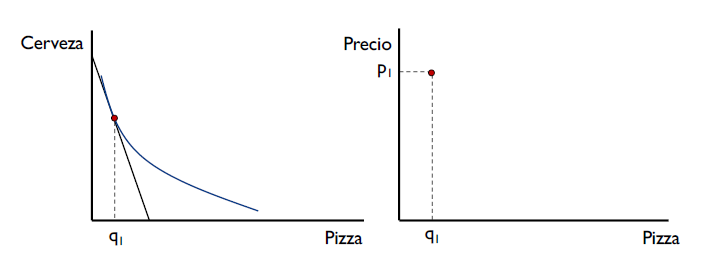
\includegraphics[scale=0.6]{Figures/Tema_02.53_derivacioncurvademanda.png}
\end{frame}

\begin{frame}
\frametitle{ Ahora el precio es P_2 \\ $P_2 < P_1 $ }
\centering
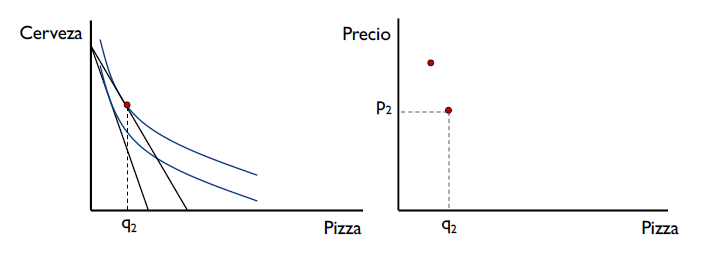
\includegraphics[scale=0.6]{Figures/Tema_02.54_derivacioncurvademanda1.png}
\end{frame}

\begin{frame}
\frametitle{ Ahora el precio es P_3 \\ $P_3 < P_2 $}
\centering
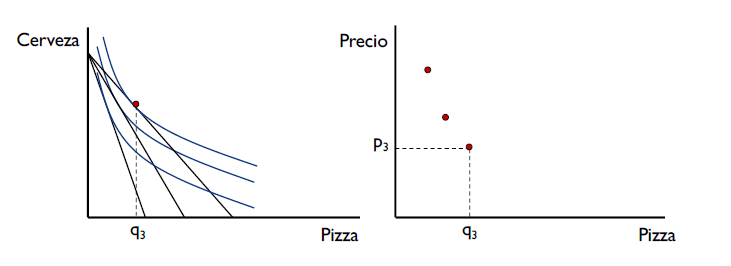
\includegraphics[scale=0.6]{Figures/Tema_02.55_derivacioncurvademanda2.png}
\end{frame}

\begin{frame}
\frametitle{ Y si seguimos asi...}
\centering
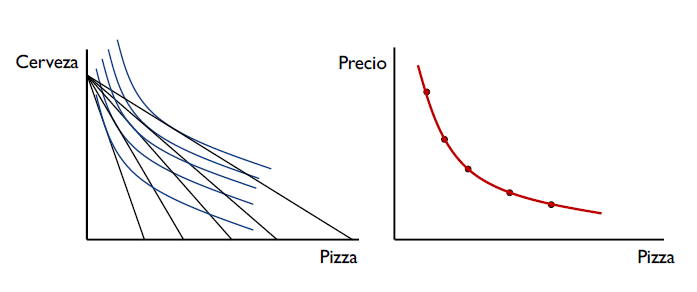
\includegraphics[scale=0.6]{Figures/Tema_02.56_derivacioncurvademanda3.png}
\end{frame}

\begin{frame}
\frametitle{¡¡¡Obtenemos la curva de demanda del estudiante!!!}
\centering
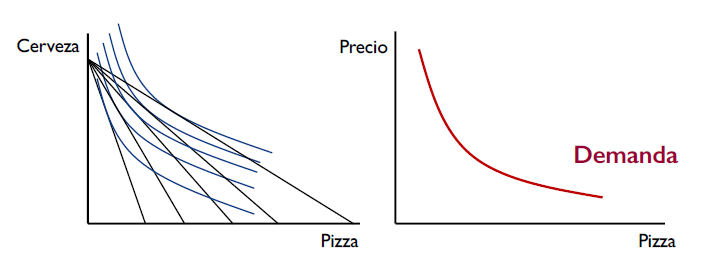
\includegraphics[scale=0.6]{Figures/Tema_02.57_derivacioncurvademanda4.png}
\end{frame}

\begin{frame}
\frametitle{ ¿Cómo pasamos de la curva de demanda individual a la curva de demanda del mercado?}

\end{frame}

\begin{frame}
\frametitle{Curva de demanda del mercado}
\centering
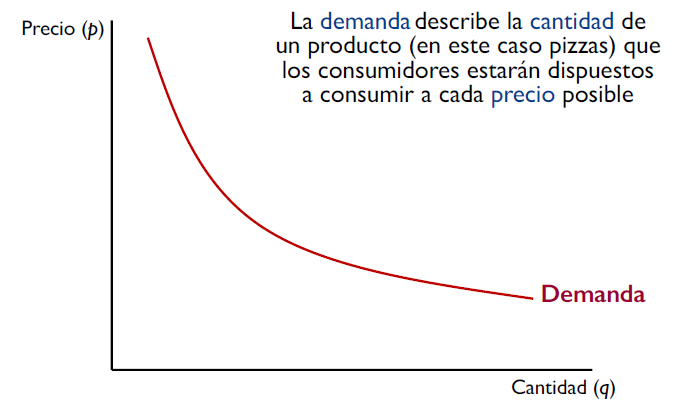
\includegraphics[scale=0.6]{Figures/Tema_02.58_demanda.png}
\end{frame}

\begin{frame}
\frametitle{¿Qué es la demanda?}
\begin{itemize}
    \item La curva de demanda muestra cuál es la disposición máxima a pagar de los consumidores para cada cantidad del bien, o
    \item cuál es la cantidad máxima del bien que está dispuesto a consumir el individuo a cada precio
\end{itemize}
\end{frame}


\end{document}
